\section{Phần chung}
\subsection{Các câu lệnh tạo bảng và ràng buộc}
\lstinputlisting{files/db_ass2.sql}
\subsection{Các câu lệnh tạo chỉ mục}
\begin{lstlisting}
create INDEX compIndex
on COMPANY (ID);

create INDEX packIndex
on PACK (ID);

create INDEX purchaseIndex
on PURCHASE(ID_COMP,ID_PACK);
\end{lstlisting}
\subsection{Các câu lệnh insert dữ liệu (nếu có)}
\newpage
\section{Phần riêng}
\subsection{Thành viên 1}
\textbf{$\indent$Thành viên 1: \\
$\indent$Họ tên: Cao Nguyệt Minh \\ 	$\indent$MSSV: 1710188}
$\indent$
\subsubsection{Thủ tục insert dữ liệu:}
\textbf{Thủ tục insert 1:}\\
$\indent$Mô tả chức năng: Tạo tài khoản cho người dùng\\
$\indent$Câu lệnh tạo thủ tục:
\lstinputlisting{files/insertUser.sql}
$\indent$Câu lệnh thực thi thủ tục mẫu: 
\begin{lstlisting}
EXEC InsertUser 'Cao Nguyet Minh', 'minh.nguyet', '123456', '1', '09-29-1999', 3
\end{lstlisting}
\newpage
\textbf{Thủ tục insert 2:}\\
$\indent$Mô tả chức năng: Tài khoản công ty tự tạo thông tin cho công ty.\\
$\indent$Câu lệnh tạo thủ tục:
\lstinputlisting{files/insertCompany.sql}
$\indent$Câu lệnh thực thi thủ tục mẫu: 
\begin{lstlisting}
EXEC InsertCompany 2, 'HCM City', 'Shopee', 'Shopee', 'JavaScript, Java, PHP, HTML5, Android, iOS', 'Shopee is the leading e-commerce platform in Southeast Asia and Taiwan.','2019-12-09',0,'assets/img/logo-default.png', '19001221',6
\end{lstlisting}
\newpage
\subsubsection{Trigger:}
\textbf{Trigger 1}\\
Mô tả chức năng: Kiểm tra thông tin của User. \\Nếu họ và tên của người dùng đều là chuỗi số thì báo lỗi. Nếu ngày sinh vượt qua thời gian hiện tại thì báo lỗi.\\
Câu lệnh tạo Trigger:
\lstinputlisting{files/triggerNUser.sql}
Câu lệnh kiểm tra trigger hoạt động: 
\begin{lstlisting}
EXEC InsertUser 'Minh Cao', 'minhcao', '123456', '0', '12-13-2020', 3
--ERROR INVALID BIRTHDATE
\end{lstlisting}
\textbf{Trigger 2}\\
Mô tả chức năng: Kiểm tra thông tin của Company \\ Nếu tên công ty là chuỗi số thì báo lỗi. Nếu số điện thoại không phải là chuỗi số thì báo lỗi.\\
Câu lệnh tạo Trigger:
\lstinputlisting{files/TriggerCompany.sql}
Câu lệnh kiểm tra trigger hoạt động: 
\begin{lstlisting}
EXEC InsertCompany 'HCM','kmswebsite.com', '21381023801', 'PHP, JavaScript', 'KMS', './assets/img/logo-company/4_logo.jpg','0929554321', 5
--Error: wrong format name
\end{lstlisting}
\subsubsection{Thủ tục chứa câu SQL:}
\textbf{Procedure 1}\\
$\indent$Mô tả chức năng: Tìm tất cả các bài tin tuyển dụng \\
$\indent$Câu lệnh tạo thủ tục:
\lstinputlisting{files/ProcedureFindRequirement.sql}
$\indent$Câu lệnh thực thi thủ tục: 
\begin{lstlisting}
EXEC findCompanyOfRequirement 'Full time'
\end{lstlisting}
\textbf{Procedure 2}\\
$\indent$Mô tả chức năng: Hiển thị thông tin chi tiết của một công ty theo ID \\
$\indent$Câu lệnh tạo thủ tục:
\lstinputlisting{files/ProcedureCompanyDetails.sql}
$\indent$Câu lệnh thực thi thủ tục: 
\begin{lstlisting}
EXEC findCompanyDetails 1
\end{lstlisting}
\subsubsection{Hàm:}
\textbf{Function 1}\\
$\indent$Mô tả chức năng: Tìm kiếm tất cả bài tin tuyển dụng của công ty đó mà người đăng tin đăng lên.\\
$\indent$Câu lệnh tạo hàm:
\lstinputlisting{files/FunctionF_RPOST_INFO.sql}
$\indent$Câu lệnh SELECT minh họa gọi hàm: 
\begin{lstlisting}
SELECT * FROM F_RPOST_INFO(1)
SELECT * FROM F_RPOST_INFO(2)
\end{lstlisting}
\textbf{Function 2}\\
$\indent$Mô tả chức năng: Tìm kiếm tất cả công ty có tên tương tự keyword và address giống location.\\
$\indent$Câu lệnh tạo hàm:
\lstinputlisting{files/FunctionSearchLocation.sql}
$\indent$Câu lệnh SELECT minh họa gọi hàm: 
\begin{lstlisting}
SELECT * FROM SearchLocation('%%','%HCM%')
SELECT * FROM SearchLocation('%Shopee%','%HCM%')
\end{lstlisting}
\subsubsection{Giao diện ứng dụng và các hình ảnh minh họa:}
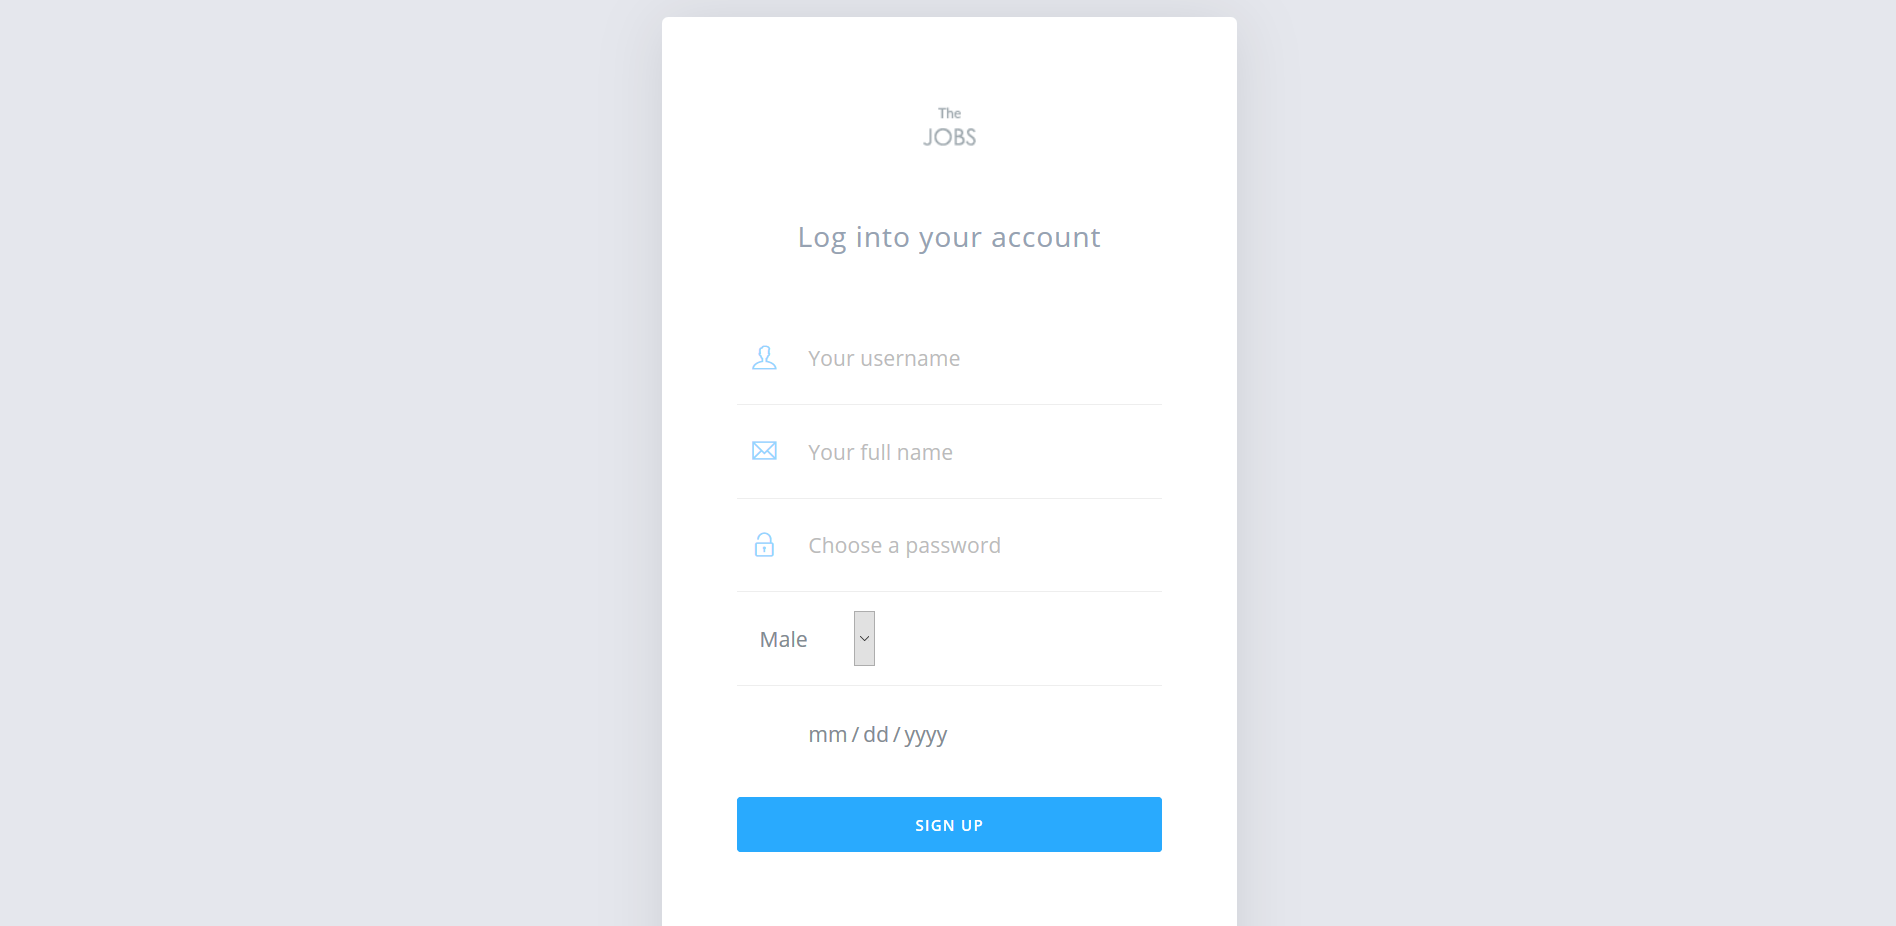
\includegraphics[width=15cm]{Images/Minh_1.png}
\vspace{0.5cm}
\newpage
\subsection{Thành viên 2}
\textbf{$\indent$Thành viên 2: \\
	$\indent$Họ tên: Nguyễn Ngọc Phát \\ 	$\indent$MSSV: 1710228}
$\indent$
\subsubsection{Thủ tục insert dữ liệu:}
$\indent$Mô tả chức năng\\
$\indent$Câu lệnh tạo thủ tục\\
$\indent$Câu lệnh thực thi thủ tục mẫu: \\
\subsubsection{Trigger:}
$\indent$Mô tả chức năng\\
$\indent$Câu lệnh tạo Trigger\\
$\indent$Câu lệnh kiểm tra trigger hoạt động: \\
\subsubsection{Thủ tục chứa câu SQL:}
$\indent$Mô tả chức năng\\
$\indent$Câu lệnh tạo thủ tục\\
$\indent$Câu lệnh thực thi thủ tục: \\
\subsubsection{Hàm:}
$\indent$Mô tả chức năng\\
$\indent$Câu lệnh tạo hàm\\
$\indent$Câu lệnh SELECT minh họa gọi hàm: \\
\subsubsection{Giao diện ứng dụng và các hình ảnh minh họa:}
$\indent$Giao diện\\
\newpage
\subsection{Thành viên 3}
\textbf{$\indent$Thành viên 3: \\
	$\indent$Họ tên: Trần Chí Kiệt \\ 	$\indent$MSSV: }
$\indent$
\subsubsection{Thủ tục insert dữ liệu:}
$\indent$Mô tả chức năng\\
$\indent$Câu lệnh tạo thủ tục\\
$\indent$Câu lệnh thực thi thủ tục mẫu: \\
\subsubsection{Trigger:}
$\indent$Mô tả chức năng\\
$\indent$Câu lệnh tạo Trigger\\
$\indent$Câu lệnh kiểm tra trigger hoạt động: \\
\subsubsection{Thủ tục chứa câu SQL:}
$\indent$Mô tả chức năng\\
$\indent$Câu lệnh tạo thủ tục\\
$\indent$Câu lệnh thực thi thủ tục: \\
\subsubsection{Hàm:}
$\indent$Mô tả chức năng\\
$\indent$Câu lệnh tạo hàm\\
$\indent$Câu lệnh SELECT minh họa gọi hàm: \\
\subsubsection{Giao diện ứng dụng và các hình ảnh minh họa:}
$\indent$Giao diện\\
\newpage
\subsection{Thành viên 3}
\textbf{$\indent$Thành viên 4: \\
	$\indent$Họ tên:  \\ 	$\indent$MSSV: }
$\indent$
\subsubsection{Thủ tục insert dữ liệu:}
$\indent$Mô tả chức năng\\
$\indent$Câu lệnh tạo thủ tục\\
$\indent$Câu lệnh thực thi thủ tục mẫu: \\
\subsubsection{Trigger:}
$\indent$Mô tả chức năng\\
$\indent$Câu lệnh tạo Trigger\\
$\indent$Câu lệnh kiểm tra trigger hoạt động: \\
\subsubsection{Thủ tục chứa câu SQL:}
$\indent$Mô tả chức năng\\
$\indent$Câu lệnh tạo thủ tục\\
$\indent$Câu lệnh thực thi thủ tục: \\
\subsubsection{Hàm:}
$\indent$Mô tả chức năng\\
$\indent$Câu lệnh tạo hàm\\
$\indent$Câu lệnh SELECT minh họa gọi hàm: \\
\subsubsection{Giao diện ứng dụng và các hình ảnh minh họa:}
$\indent$Giao diện\\
\newpage
\subsection{Thành viên 5}
\textbf{$\indent$Thành viên 5: \\
	$\indent$Họ tên: \\ 	$\indent$MSSV: }
\subsubsection{Thủ tục insert dữ liệu:}
$\indent$Mô tả chức năng\\
$\indent$Câu lệnh tạo thủ tục\\
$\indent$Câu lệnh thực thi thủ tục mẫu: \\
\subsubsection{Trigger:}
$\indent$Mô tả chức năng\\
$\indent$Câu lệnh tạo Trigger\\
$\indent$Câu lệnh kiểm tra trigger hoạt động: \\
\subsubsection{Thủ tục chứa câu SQL:}
$\indent$Mô tả chức năng\\
$\indent$Câu lệnh tạo thủ tục\\
$\indent$Câu lệnh thực thi thủ tục: \\
\subsubsection{Hàm:}
$\indent$Mô tả chức năng\\
$\indent$Câu lệnh tạo hàm\\
$\indent$Câu lệnh SELECT minh họa gọi hàm: \\
\subsubsection{Giao diện ứng dụng và các hình ảnh minh họa:}
$\indent$Giao diện\\
\section{Phụ lục}
\subsection{Báo cáo bài tập lớn 1}
\newpage
\subsubsection{Lược đồ (E-)ERD}
\newpage
\subsubsection{Ánh xạ sang lược đồ CSDL}
\newpage
\subsection{Source code chương trình:}
\subsection{Bảng phân công nhiệm vụ cho phần chung và bài tập lớn số 1}
\begin{center}
	\begin{tabular}{ | m{4cm} | m{10cm}|  } 
		\hline
		\textbf{Họ và tên}&\textbf{Phân công công việc  } \\ 
		\hline
		Cao Nguyệt Minh & - Vẽ ERRD (BTL1), viết câu lệnh insert dữ liệu, viết backend\\ 
		\hline
		Nguyễn Ngọc Phát & - Vẽ ERRD (BTL1), viết câu lệnh tạo bảng, viết backend\\
		\hline
		Trần Chí Kiệt & - Viết câu lệnh tạo bảng \\
		\hline
		Cao Minh Khôi & - Viết câu lệnh tạo bảng, tạo chỉ mục \\
		\hline
		Cao Ngọc Xuân Yến & - Viết câu lệnh insert dữ liệu \\
		\hline
	\end{tabular}
\end{center}
\newpage
\end{document}


